% Slide 2 | Model and E1 | M3 (Tanishk Tasgaonkar) | 2:30 | OU model, exact step, E1
\begin{frame}{The OU model, and how well its speed $\kappa$ can be estimated}
\framesubtitle{Slide 2 \textbullet\ Model and E1 \textbullet\ Tanishk \textbullet\ 2:30}
\vspace{-2pt}
\begin{columns}[T,onlytextwidth]
\column{0.47\textwidth}
  \small\raggedright
  \textbf{\color{deckAccent}The spread}
  \[ dX_t=\kappa(\theta-X_t)\,dt+\sigma\,dW_t \]
  \textbf{\color{deckAccent}Exact daily step}\ {\footnotesize($\Delta=1/252$)}
  \[ X_{t+\Delta}=a+bX_t+\varepsilon_t,\quad b=e^{-\kappa\Delta} \]
  \[ \hat\kappa=-\frac{\ln\hat b}{\Delta} \]
  \begin{itemize}\setlength{\itemsep}{2pt}
    \item $\kappa$ speed, $\theta$ level, $\sigma$ noise
    \item an AR(1), so least squares is maximum likelihood
  \end{itemize}
\column{0.50\textwidth}
  \centering
  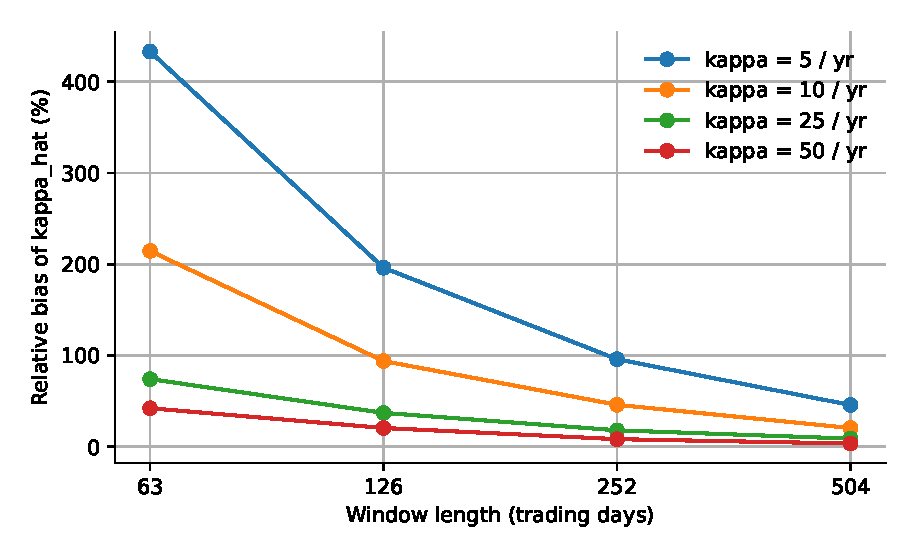
\includegraphics[width=\linewidth]{fig_e1_ou_estimation}\\[2pt]
  \footnotesize\raggedright
  \textbf{E1:} with one year of data $\hat\kappa$ is too high by \textbf{18\%} (7-day half-life) and \textbf{96\%} (35-day); the error halves when the window doubles
\end{columns}
\pairTakeaway{Pairs look faster, and more attractive, than they really are.}
\end{frame}
